% Faithful initial reconstruction of Clause 9 from source PDF pages 199--226
% (standard pages 185--212). Source-page boundaries are intentionally preserved.

\clearpage

% --- Standard page 185 / source PDF page 199 ---
\begin{compactstdpage}

    \section{Data distribution management (DDM)}

    \subsection{Overview}

    DDM services may be used by joined federates to reduce both the transmission and the reception of irrelevant data. Whereas DM services provide information on data relevance at the class attribute level, DDM services add the capability to further refine the data requirements at the instance attribute level. Similarly, whereas DM services provide information on data relevance at the interaction class level, DDM services add the capability to further refine the data requirements at the specific interaction level. Producers and consumers of data communicated between joined federates may use the DDM services to bound the relevance of such communicated data. As a result, the RTI can recognize the irrelevant data and prevent its delivery to consumers. The relevance of communicating interactions or instance attribute updates is expressed by giving a bounding for relevant communication in a space of user-defined dimensions. Both consumers and producers specify the upper and lower bounds for the relevant portion of that space, and the overlap of producers' and consumers' region sets is used to bound relevant communication.

    \subsubsection{Definitions for DDM}

    The DDM services shall be based on the following concepts and terms:

    \stdliteralitem{a)}{A dimension shall be a named interval of nonnegative integers. The interval shall be defined by an ordered pair of values. The first value is 0 (zero) for every dimension. The second value, which can vary for each dimension, is that dimension's upper bound as specified in the FDD.}
    \stdliteralitem{b)}{A range shall be a continuous semi-open interval on a dimension. The interval is defined by an ordered pair of values. The first component of the pair shall be called range lower bound, and the second component shall be called range upper bound. The range upper bound shall be strictly greater than the range lower bound. The minimum possible difference between a range lower bound and a range upper bound shall be 1 (one).}
    \stdliteralitem{c)}{A region specification shall be a set of ranges. The dimensions contained in a region specification shall be the dimensions of the ranges that are included in the region specification. A region specification shall contain at most one range for any given dimension. Each range in a region specification shall be defined in terms of the bounds [0, the corresponding dimension's upper bound).}
    \stdliteralitem{d)}{A region template shall be an incomplete region specification where one or more dimensions have not been assigned ranges.}
    \stdliteralitem{e)}{A region realization shall be a region specification that is associated with an instance attribute for update, with a sent interaction or with a class attribute or interaction class for subscription. The generic term region may be used in circumstances where a region specification, a region realization, or both apply.}
    \stdliteralitem{f)}{The RTI shall provide the default region, which is defined as having the range [0, the range's dimension's upper bound) for each dimension found in the FDD. The default region shall have all dimensions found in the FDD, regardless of the class attribute or interaction class with which it is associated. The default region realization shall not have a region specification. There shall be no way for a joined federate to refer to the default region. If a joined federate creates a region that has as its dimensions all dimensions found in the FDD and has the range [0, the range's dimension's upper bound) for each dimension, this region shall be equivalent to the default region, but it is not the default region.}
    \stdliteralitem{g)}{A collection of attribute designator set and region designator set pairs shall be interpreted as a set of (attribute designator, region designator) pairs. The interpreted form can be viewed as if constructed in the following manner:}
    \stdliteralsubitem{1)}{The interpreted form begins as an empty set of (attribute designator, region designator) pairs.}
    \stdliteralsubitem{2)}{For each pair (of sets) in the attribute designator set and region designator set pair collection, create the cross product of the attribute designator set with its region designator set. The result}

\end{compactstdpage}

\clearpage

% --- Standard page 186 / source PDF page 200 ---
\begin{compactstdpage}

    is a collection of (attribute designator, region designator) pairs. The union of all such (attribute designator, region designator) pairs shall be the interpreted form.

    Some DDM services require that the region designator used as an argument be the designator of a region specification, whereas other DDM services require that the region designator used as an argument be the designator of either a region template or a region specification. One DDM service, Commit Region Modifications, requires that the region designator used as an argument be that of either a region template that has had the Set Range Bounds service called at least once for all of its dimensions or a region specification. If a DDM or Support service is invoked with a region designator argument that is not of the variety it is expecting, the service shall throw the ``Invalid region'' exception. Hence, the circumstances that shall cause the ``Invalid region'' exception to be thrown vary from service to service, depending on the type of region entity (template, specification, or template with all range bounds set) for which the service is expected to receive a designator.

    For all services that can be used to create a region realization from a region specification, the region designator argument shall be the designator of a region specification. Specifically, the following services, which result in the creation of region realizations from region specifications, require that the region designator argument be the designator of a region specification: Register Object Instance With Regions, Associate Regions For Updates, Subscribe Object Class Attributes With Regions, Subscribe Interaction Class With Regions, Send Interaction With Regions, and Request Attribute Value Update With Regions.

    The following services also require that the region designator argument be the designator of a region specification: Unassociate Regions for Updates, Unsubscribe Object Class Attributes With Regions, and Unsubscribe Interaction Class With Regions.

    The region designator argument for the Delete Region service shall be the designator of either a region template or a region specification.

    There are also three Support services that take a region designator as argument:

    \stdliteraldashitem{The region designator argument for the Get Range Bounds service shall be the designator of either a region specification or a region realization.}
    \stdliteraldashitem{The region designator argument for the Get Dimension Handle Set service shall be the designator of a region template, a region specification, or a region realization.}
    \stdliteraldashitem{The region designator argument for the Set Range Bounds service shall be the designator of either a region template or a region specification.}

    \subsubsection{Relating region specifications and region realizations}

    The following relationships, established in the FDD, shall pertain to dimensions:

    \stdliteralitem{a)}{The available dimensions of a class attribute shall be the dimensions associated with that class attribute in the FDD. The available dimensions of an instance attribute shall be the available dimensions of the corresponding class attribute.}
    \stdliteralitem{b)}{The available dimensions of an interaction class shall be the dimensions associated with that class in the FDD. The available dimensions of a sent interaction shall be the available dimensions of the interaction class specified in the Send Interaction With Regions service invocation.}
    \stdliteralitem{c)}{DDM services shall not be invoked for class attributes, instance attributes, interaction classes, or sent interactions that do not have available dimensions.}
    \stdliteralitem{d)}{Each dimension in the FDD shall have either a default range specified in terms of the bounds [0, the dimension's upper bound) or shall have an excluded indicator specified in the Value When Unspecified Field of the FDD Dimension Table. Where a default range is specified for a dimension in the FDD and the dimension is not mentioned in a region specification, it is implicitly added, with the specified default range, when creating a region realization.}

\end{compactstdpage}

\clearpage

% --- Standard page 187 / source PDF page 201 ---
\begin{compactstdpage}

    \subsubsection{Using regions}

    \paragraph{Region relationships}

    The following relationships, established through DDM services, shall pertain to regions:

    \stdliteralitem{a)}{The only way that a region specification can be created is by a federate successfully invoking the following services, in order:}
    \stdliteralsubitem{1)}{Invoke the Create Region service (see 9.2) to create a region with a specific set of dimensions.}
    \stdliteralsubitem{2)}{For every dimension that was explicitly specified when that region was created, invoke the Set Range Bounds service (see 10.32) to set the lower and upper bounds of the range of that dimension for that region.}
    \stdliteralsubitem{3)}{Invoke Commit Region Modifications (see 9.3) to inform the RTI about the changes to the ranges of the dimensions specified in the preceding series of Set Range Bounds service invocations.}
    A region template is created when a federate invokes the Create Region service. The region designator argument that is returned as a result of the Create Region service is a designator of a region template only. It is not the designator of a region specification because the range bounds have not yet been set for all of the dimensions of the region template followed by a successful invocation of the Commit Region Modifications service for this region. Only after the Set Range Bounds service has been successfully invoked for every dimension in the region, followed by a successful invocation of the Commit Region Modifications service, is that region designator the designator of a region specification.

    \stdliteralitem{b)}{When a federate invokes the Register Object Instance With Region, Associate Regions For Updates, Subscribe Object Class Attributes With Regions, Subscribe Interaction Class With Regions, Send Interaction With Regions, or Request Attribute Value Update With Regions service with that region specification designator as an argument, one or more region realizations are created. These region realizations, however, do not have designators.}
    \stdliteralitem{c)}{The specified dimensions of the region specification shall be the dimensions that are explicitly provided when the Create Region service is invoked to create that region specification. Invocation of neither the Set Range Bounds service nor the Commit Region Modifications service for a particular region has any effect on what the specified dimensions of that region specification are.}
    \stdliteralitem{d)}{The unspecified dimensions of a region realization shall be the available dimensions of the class attribute, instance attribute, interaction class, or sent interaction with which the region realization is associated less the specified dimensions of the region specification from which the region realization is derived.}
    \stdliteralitem{e)}{The Commit Region Modifications service can only either}
    \stdliteralsubitem{1)}{Create a region specification from a region template, or}
    \stdliteralsubitem{2)}{Modify the range bounds of an existing region specification and thereby also modify the range bounds of all existing region realizations that are derived from that region specification.}
    \stdliteralitem{f)}{When a region realization is created by associating a region specification with an instance attribute, a class attribute, an interaction class, or a sent interaction, additions may be made to the region realization by the RTI to account for default dimension values indicated in the FDD as follows:}
    \stdliteralsubitem{1)}{All specified dimensions of the region specification shall be included in the region realization, and the range associated with each specified dimension in the region realization shall be the range found in the region specification for the same dimension.}
    \stdliteralsubitem{2)}{For each unspecified dimension of the region realization, if the FDD indicates a default range other than the excluded indicator, this default range shall be added to the region realization.}
    \stdliteralsubitem{3)}{When a federate modifies a region specification from which region realizations have been derived, the RTI shall fill in unspecified dimensions in the region realizations in this same manner.}

\end{compactstdpage}

\clearpage

% --- Standard page 188 / source PDF page 202 ---
\begin{compactstdpage}

    \stdliteralitem{g)}{A region specification may contain an empty set of ranges. The region realization derived from such a region specification shall contain only the dimensions for which the FDD defines a default range and that are available dimensions of the instance attribute, class attribute, interaction class, or sent interaction with which the region specification is being associated. This situation may result in a region realization that contains no dimensions if all available dimensions have the excluded indicator specified in the FDD; such a region realization shall not overlap with any other region realization, even the default region.}
    If a federate invokes the Create Region service but does not subsequently successfully invoke the Set Range Bounds service for every dimension in the region, followed by a successful invocation of the Commit Region Modifications service for the region, then the federate has not created a region specification. In particular,

    \stdliteralitem{h)}{If a federate invokes the Create Region service and then does not invoke the Set Range Bounds service or invokes the Set Range Bounds service for only some, but not all, of the dimensions that were specified when the region was created, followed by an invocation of the Commit Region Modifications service for that region, the Commit Region Modifications service shall throw the ``Invalid region'' exception because each region designator that is passed to the Commit Region Modifications service is required to have had the Set Range Bounds service invoked at least once for all of its dimensions. The effects of the Set Range Bounds service invocations that were made, if any, are still pending. They shall take effect if and when the Set Range Bounds service has been invoked at least once for all of the dimensions of the region, followed by the invocation of the Commit Region Modifications service for that region.}
    \stdliteralitem{i)}{If a federate invokes the Create Region service, followed by at least one Set Range Bounds service invocation for every one of the dimensions that were specified when the region was created, but does not invoke the Commit Region Modifications service, the region continues to be only a region template, not a region specification. The effects of the Set Range Bounds service invocations are still pending and shall take effect if and when the Commit Region Modifications service is successfully invoked for that region.}
    The effects of invocation of the Set Range Bounds service for a given region (template or specification) shall remain pending until the Commit Region Modifications service is subsequently invoked for that region. If a federate invokes the Set Range Bounds service repeatedly for a given dimension of a given region before invoking the Commit Region Modifications service for that region, the range values provided in the most recent invocation of the Set Range Bounds service shall become the range values for that dimension of that region specification.

    \paragraph{Instance attribute relationships}

    The following relationships, established through DDM services, shall pertain to object classes, class attributes, object instances, and instance attributes:

    \stdliteralitem{a)}{A region realization other than the default region shall be used for update of an instance attribute if the joined federate owns the instance attribute and has used the instance attribute and region specification from which the region realization was derived as arguments either in the Register Object Instance With Regions service or in the Associate Regions For Updates service. The default region shall be used for update of an instance attribute if and only if the corresponding class attribute has available dimensions and there is no other region realization used for update for that instance attribute. This situation may occur if the Register Object Instance service is used to register an instance of an object class that has attributes with available dimensions or if a region association for update is removed via the Unassociate Regions for Updates service.}

\end{compactstdpage}

\clearpage

% --- Standard page 189 / source PDF page 203 ---
\begin{compactstdpage}

    Subsequently invoking the Unassociate Regions For Updates service for the same (object instance, region, attribute) triple shall cause that region not to be used for update of that instance attribute. Invoking the Associate Regions For Updates service or the Unassociate Regions For Updates service with an empty set of regions shall make no changes to the set of associations of the instance attribute. Any region specifications used to generate region realizations associated with an instance attribute for update shall contain only dimensions that are a subset of the available dimensions of that instance attribute. The resulting region realizations shall have the same property. A joined federate shall use a region for update of an instance attribute to assert properties of that instance attribute. These properties shall be used to limit reflection of the instance attributes when the joined federate invokes the Update Attribute Values service. If a region other than the default region is used for update of a particular instance attribute by a joined federate and the joined federate loses ownership of that instance attribute, that region shall no longer be used for update of that instance attribute. A joined federate may create and modify update region associations with an instance attribute that is owned by another joined federate or that is unowned. These associations shall not take effect until the joined federate making the associations has acquired ownership of the specified instance attribute. These associations shall take effect immediately upon acquiring ownership of the specified instance attributes. In all cases, if a joined federate divests ownership of an instance attribute with which an update region is associated, that association shall be lost, as if the Unassociate Regions For Updates service had been invoked for that (object instance, region, attribute) triple. Update region associations that are lost shall not come into effect if the joined federate subsequently acquires ownership of the instance attribute unless the joined federate explicitly recreates the association.

    \stdliteralitem{b)}{A region realization other than the default region shall be used for subscription of a class attribute if the joined federate has used the class attribute and a given object class and the region specification from which the region realization was derived as arguments in the Subscribe Object Class Attributes With Regions service. Subsequently invoking the Unsubscribe Object Class Attributes With Regions service for the same (object class, region, attribute) triple shall cause the region not to be used for subscription of that class attribute. Invoking the Subscribe Object Class Attributes With Regions service or the Unsubscribe Object Class Attributes With Regions service with an empty set of regions shall make no changes to the set of subscriptions with region of the class attribute. Any region specifications used to generate region realizations associated with a class attribute for subscription shall contain only dimensions that are a subset of the available dimensions of that class attribute. The resulting region realizations shall have the same property. The default region shall be used for subscription of a class attribute if and only if that class attribute has available dimensions, there is no other region realization used for subscription of that class attribute, and the joined federate is subscribed to that class attribute. Subsequently invoking the Unsubscribe Object Class Attributes service for the same object class and attribute shall cause the default region not to be used for subscription of that class attribute. A joined federate shall use a region for subscription of a class attribute to specify requirements for reflecting values of that class attribute's analogous instance attributes.}

\end{compactstdpage}

\clearpage

% --- Standard page 190 / source PDF page 204 ---
\begin{compactstdpage}

    \paragraph{Interaction relationships}

    The following relationships, established through DDM services, shall pertain to interaction classes, parameters, and interactions:

    \stdliteralitem{a)}{A region realization other than the default region shall be used for sending an interaction if the joined federate has used the interaction and a region specification from which the region realization may be derived as arguments to an invocation of the Send Interaction With Regions service. Any region associated with a sent interaction shall contain only dimensions that are a subset of the available dimensions of the sent interaction. The default region shall be used for sending an interaction of such a class during an invocation of the Send Interaction service. A joined federate shall use a region for sending an interaction to assert properties of that interaction when the Send Interaction With Regions service is invoked.}
    \stdliteralitem{b)}{A region realization other than the default region shall be used for subscription of an interaction class if the joined federate has used the interaction class and the region specification from which the region realization was derived as arguments in the Subscribe Interaction Class With Regions service. Subsequently invoking the Unsubscribe Interaction Class With Regions service for the same (interaction class, region) pair shall cause the region not to be used for subscription of that interaction class. Invoking the Subscribe Interaction Class With Regions service or the Unsubscribe Interaction Class With Regions service with an empty set of regions shall make no changes to the set of subscriptions with region of the interaction class. Any region associated with an interaction class for subscription shall contain only dimensions that are a subset of the available dimensions of that interaction class. The default region shall be used for subscription of that interaction class if and only if that interaction class has available dimensions, there is no other region realization used for subscription of that interaction class, and the joined federate is subscribed to that interaction class. Subsequently invoking the Unsubscribe Interaction Class service for the same interaction class shall cause the default region not to be used for subscription of that interaction class. A joined federate shall use a region for subscription of an interaction class to establish requirements for receiving interactions of that class.}
    A set of region realizations used for update of instance attributes or for sending interactions shall be called an \textbf{update region set}.

    A set of region realizations used for subscription of either class attributes or interaction classes shall be called a \textbf{subscription region set}.

    \subsubsection{Calculating region overlaps}

    An update region set and a subscription region set shall overlap if and only if a region exists in each set so that the two regions overlap. Two regions overlap if and only if all ranges of dimensions that are contained in both regions overlap pairwise. If two regions do not have any dimensions in common, they shall not overlap. Two ranges in the same dimension $A = [a_{\mathrm{lower}}, a_{\mathrm{upper}})$ and $B = [b_{\mathrm{lower}}, b_{\mathrm{upper}})$ shall overlap if and only if either $a_{\mathrm{lower}} = b_{\mathrm{lower}}$ or $(a_{\mathrm{lower}} < b_{\mathrm{upper}}$ and $b_{\mathrm{lower}} < a_{\mathrm{upper}})$. The default region shall overlap with all nonempty region realizations.

    The normalization of federation data to [0, a particular dimension's upper bound) for use with DDM services shall be left to the federation. The effects of DDM services shall be independent of the HLA time axis and HLA time management services.

    Figure 18 depicts a region with two dimensions.

\end{compactstdpage}

\clearpage

% --- Standard page 191 / source PDF page 205 ---
\begin{compactstdpage}

    \vspace*{3pt}
    \begin{center}
        \hspace*{-1.7pt}% Figure 18 - Region of two dimensions
% Independently revalidated against IEEE Std 1516.1-2010 source physical p.205.
% Natural source raster: 784 x 498, placed anisotropically at
% (116.8405,75.4163)..(491.7395,305.7828) PDF pt.
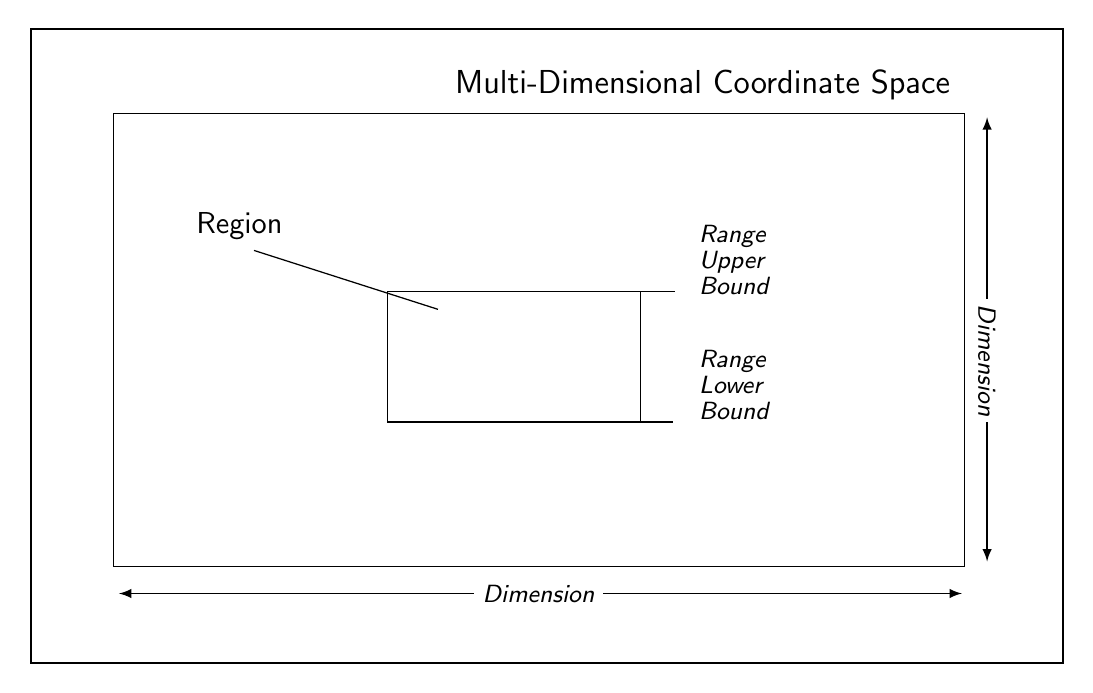
\begin{tikzpicture}[x=.4781875221pt,y=-.4625833350pt,line cap=butt,line join=miter,>=latex]
    \path[use as bounding box] (0,0) rectangle (784,498);

    % Source PDF draws this outside the one-bit figure image; included natively here.
    \draw[line width=.72pt] (2.22,1.05) rectangle (782.16,496.53);

    % Multi-dimensional coordinate-space box.
    \draw[line width=.45pt] (65,67) rectangle (708,421);
    \node[anchor=center,font=\sffamily\fontsize{11.5}{12.2}\selectfont] at (510,45)
        {Multi-Dimensional Coordinate Space};

    % Region realization.
    \draw[line width=.45pt] (272,206) rectangle (463,308);
    \draw[line width=.45pt] (463,206) -- (489,206);
    \draw[line width=.45pt] (463,308) -- (488,308);
    \node[anchor=center,font=\sffamily\fontsize{10.7}{11.4}\selectfont] at (160,155) {Region};
    \draw[line width=.45pt] (171,174) -- (310,220);

    % Range-bound labels.
    \node[anchor=west,align=left,font=\sffamily\itshape\fontsize{9.0}{9.4}\selectfont]
    at (500,181) {Range\\Upper\\Bound};
    \node[anchor=west,align=left,font=\sffamily\itshape\fontsize{9.0}{9.4}\selectfont]
    at (500,279) {Range\\Lower\\Bound};

    % Horizontal dimension indicator. The source line is interrupted by its label.
    \draw[line width=.55pt,<->] (69,442) -- (706,442);
    \node[fill=white,inner xsep=3.2pt,inner ysep=.2pt,
        font=\sffamily\itshape\fontsize{9.2}{9.6}\selectfont] at (386,442) {Dimension};

    % Vertical dimension indicator. The label masks the middle of the arrow line.
    \draw[line width=.55pt,<->] (725,70) -- (725,417);
    \node[fill=white,inner xsep=2.2pt,inner ysep=.3pt,rotate=-90,
        font=\sffamily\itshape\fontsize{9.2}{9.6}\selectfont] at (725,260) {Dimension};
\end{tikzpicture}

        \par\vspace{3.2pt}
        {\sffamily\bfseries\fontsize{9.0}{10.2}\selectfont Figure 18---Region of two dimensions}
    \end{center}

    \subsubsection{Reinterpretation of selected DM services}

    Some DDM services can be used to perform similar functions to what is accomplished with DM services. When a joined federate uses DDM services, some of the DM definitions, constraints and services described in Clause 6 shall be extended to encompass the expanded interpretation of how DM services work when used in conjunction with DDM services by a joined federate, from the perspective of that joined federate.

    A joined federate that is using DDM services shall interpret all uses of the following four DM services by any joined federate (including itself) in the federation execution:

    \stdliteraldashitem{\emph{Subscribe Object Class Attributes}}
    \stdliteraldashitem{\emph{Unsubscribe Object Class Attributes}}
    \stdliteraldashitem{\emph{Subscribe Interaction Class}}
    \stdliteraldashitem{\emph{Unsubscribe Interaction Class}}
    as special cases of the following DDM services, respectively:

    \stdliteraldashitem{\emph{Subscribe Object Class Attributes With Regions}}
    \stdliteraldashitem{\emph{Unsubscribe Object Class Attributes With Regions}}
    \stdliteraldashitem{\emph{Subscribe Interaction Class With Regions}}
    \stdliteraldashitem{\emph{Unsubscribe Interaction Class With Regions}}
    From the perspective of the joined federate that is using DDM services, each of the four DM services listed above shall be defined to be equivalent to the corresponding DDM service when invoked with a region argument of the default region.

    In practice, because there shall be no way to refer to the default region, there shall be no way to substitute a DDM service for its corresponding DM service. Furthermore, a given joined federate may invoke both the DM services listed above and their corresponding DDM services using the same object class and class attribute designators or interaction class designators as arguments and there shall be no interaction between


\end{compactstdpage}

\clearpage

% --- Standard page 192 / source PDF page 206 ---
\begin{compactstdpage}

    the subscription effects that result from the DM service invocations and those that result from the DDM service invocations.

    For a joined federate that is using DDM services, the following expanded definitions and constraints shall replace the correspondingly numbered DM definitions and constraints that appear in 5.1.2 and 5.1.3.

    Expanded definitions and constraints replace corresponding items in 5.1.2 as follows:

    \stdliteralitem{a)}{A class attribute may be used as an argument to Subscribe Object Class Attributes, Subscribe Object Class Attributes With Regions, Unsubscribe Object Class Attributes, Unsubscribe Object Class Attributes With Regions, Publish Object Class Attributes, and Unpublish Object Class Attributes service invocations for a particular object class if and only if the attribute is an available attribute of that object class.}
    \stdliteralitem{b)}{From a joined federate's perspective, the subscribed attributes of an object class shall be all of the class attributes that have been arguments to Subscribe Object Class Attributes service invocations by that joined federate for that object class and that have not subsequently been unsubscribed, either individually or by unsubscribing the whole object class. Subscribe Object Class Attributes and Unsubscribe Object Class Attributes service invocations for one object class shall have no effect on the subscribed attributes of any other object class. From a joined federate's perspective, the subscribed attributes of an object class with region shall be the class attributes that have been arguments to Subscribe Object Class Attributes With Regions service invocations by that joined federate for that object class and any region, assuming the joined federate did not subsequently invoke the Unsubscribe Object Class Attributes With Regions service for that (object class, region, class attribute) triple. Subscribe Object Class Attributes With Regions and Unsubscribe Object Class Attributes With Regions service invocations for one (object class, region, class attribute) triple shall have no effect on the subscribed attributes of any other (object class, region, class attribute) triples. Subscribe Object Class Attributes and Unsubscribe Object Class Attributes service invocations shall have no effect on any class attribute with region subscriptions that were established via the Subscribe Object Class Attributes With Regions service. Subscribe Object Class Attributes With Regions and Unsubscribe Object Class Attributes With Regions service invocations shall have no effect on any class attribute subscriptions that were established via the Subscribe Object Class Attributes service.}
    \stdliteralitem{c)}{If a class attribute is a subscribed attribute of an object class, the joined federate shall be subscribed to that class attribute either actively or passively, but not both. If a class attribute is a subscribed attribute of an object class with region, the joined federate shall be subscribed to that class attribute at a given object class and region either actively or passively, but not both.}
    \stdliteralitem{h)}{From a joined federate's perspective, an object class shall be subscribed if and only if}
    \stdliteralsubitem{1)}{The joined federate is subscribed to at least one attribute of the object class, or}
    \stdliteralsubitem{2)}{The joined federate is subscribed with region to at least one attribute of the object class.}
    \stdliteralitem{j)}{Joined federates may invoke the Register Object Instance and the Register Object Instance With Regions services only with a published object class as an argument.}
    \stdliteralitem{k)}{The registered class of an object instance shall be the object class that was an argument to either the Register Object Instance or the Register Object Instance With Regions service invocation for that object instance.}
    \stdliteralitem{s)}{An update to an instance attribute by the joined federate that owns that instance attribute may be reflected only by other joined federates that are either}
    \stdliteralsubitem{1)}{Subscribed to the instance attribute's corresponding class attribute at the known class of the object instance that contains that instance attribute at the subscribing joined federate, or}
    \stdliteralsubitem{2)}{Using a subscription region set for the instance attribute's corresponding class attribute at the known class of the object instance at the subscribing joined federate, and this set overlaps the update region set of the specified instance attribute at the wall-clock time that the Update}

\end{compactstdpage}

\clearpage

% --- Standard page 193 / source PDF page 207 ---
\begin{compactstdpage}

    Attribute Values service was invoked. An update shall be reflected at the subscribing joined federate at most once, regardless of another subscription to the class attribute using the Subscribe Object Class Attributes service.

    Expanded definitions and constraints replace corresponding items in 5.1.3 as follows:

    \stdliteralitem{a)}{From a joined federate's perspective, an interaction class shall be subscribed if and only if}
    \stdliteralsubitem{1)}{It was an argument to a Subscribe Interaction Class service invocation by that joined federate that was not subsequently followed by an Unsubscribe Interaction Class service invocation for that interaction class, or}
    \stdliteralsubitem{2)}{There is at least one region where the interaction class and region were arguments to a Subscribe Interaction Class With Regions service invocation by that joined federate that was not subsequently followed by an Unsubscribe Interaction Class With Regions service invocation for that interaction class and region.}
    \stdliteralitem{b)}{If an interaction class is subscribed, the joined federate shall be subscribed to that interaction class either actively or passively, but not both. If an interaction class is subscribed with region, the joined federate shall be subscribed to that interaction class with a given region either actively or passively, but not both.}
    \stdliteralitem{d)}{Joined federates may invoke the Send Interaction and the Send Interaction With Regions services only with a published interaction class as an argument.}
    \stdliteralitem{e)}{The sent class of an interaction shall be the interaction class that was an argument to the Send Interaction or the Send Interaction With Regions service invocation for that interaction.}
    \stdliteralitem{g)}{The Receive Interaction \rtiinitiated{} service shall be invoked at a joined federate only with a subscribed interaction class as an argument. An interaction shall be received at the joined federate at most once, regardless of another subscription to the interaction class using the Subscribe Interaction Class service.}
    \stdliteralitem{j)}{Only the available parameters of an interaction class may be used in a Send Interaction and Send Interaction With Regions service invocation with that interaction class as an argument.}
    \stdliteralitem{k)}{The sent parameters of an interaction shall be the parameters that were arguments to the Send Interaction or Send Interaction With Regions service invocation for that interaction.}

    \subsubsection{Reinterpretation of selected object management services}

    Some DDM services can be used to perform similar functions to what is accomplished with object management services. When a joined federate uses DDM services, the RTI shall extend processing of three of the object management services described in Clause 6 to encompass the expanded interpretation of how object management services work when used in conjunction with DDM services by a joined federate, from the perspective of that joined federate.

    A joined federate using DDM services shall interpret all uses of the following three object management services by any joined federate in the federation execution (including itself):

    \stdliteraldashitem{Register Object Instance}
    \stdliteraldashitem{Send Interaction}
    \stdliteraldashitem{Request Attribute Value Update}
    as special cases of the following DDM services, respectively:

    \stdliteraldashitem{Register Object Instance With Regions}
    \stdliteraldashitem{Send Interaction With Regions}
    \stdliteraldashitem{Request Attribute Value Update With Regions}

\end{compactstdpage}

\clearpage

% --- Standard page 194 / source PDF page 208 ---
\begin{compactstdpage}

    From the perspective of the joined federate that is using DDM services, each of the three object management services listed above shall be defined to be equivalent to the corresponding DDM service when invoked with a region argument of the default region.

    \subsubsection{Convey Region Designator Sets Switch}

    Each federate's Convey Region Designator Sets Switch indicates whether the RTI shall provide the optional Set of Sent Region Designators argument with invocations of Reflect Attribute Values \rtiinitiated{} and Receive Interaction \rtiinitiated{} services at the joined federate.

    The federation-wide initial setting for this switch shall come from the FDD supplied to the Create Federation Execution service invocation for the federation execution. This switch setting shall be modifiable during a federation execution via the HLAmanager.HLAfederation.HLAadjust.HLAsetSwitches MOM interaction.

    Whenever this switch is enabled at a joined federate, the optional Set of Sent Region Designators argument shall be provided (as appropriate) with all Reflect Attribute Values \rtiinitiated{} and Receive Interaction \rtiinitiated{} service invocations at that joined federates. For the Reflect Attribute Values \rtiinitiated{} service, if the specified instance attributes have available dimensions, the Set of Sent Region Designators argument shall contain the respective update region set. For the Receive Interaction \rtiinitiated{} service, if the specified interaction has available dimensions, the Set of Sent Region Designators argument shall contain the respective update region set.

    If the specified interaction or corresponding class attributes has available dimensions, this switch is enabled, and no region designator set is supplied, then the default region shall have been used on the sending side. In this case, the Convey Region set argument shall be present and empty.

    A joined federate shall use the region realization designators received in conveyed region sets only in the Get Range Bounds and Get Dimension Handle Set service invocations.

    The Set of Sent Region Designators conveyed is not a set of designators of region specifications or a set of designators of region realizations. It is, instead, a set of designators of copies of the update region realizations. The range values of each of the dimensions in each of these region realization copies are the same as the range values of each of the dimensions of the corresponding update region realization that were in effect when the region overlap calculation was performed. Each designator is guaranteed to refer to a particular region realization copy, and the copy is guaranteed to remain intact, until the Reflect Attribute Values \rtiinitiated{} service or the Receive Interaction \rtiinitiated{} service invocation at the receiving/reflecting federate completes. No change to the range values of the region realization from which the copy was made shall cause a change to the range values of the copy as long as the Reflect Attribute Values \rtiinitiated{} service or the Receive Interaction \rtiinitiated{} service invocation is still in progress.

    \subsection{Create Region service}

    The Create Region service shall create a region that has the specified dimensions. The region may be used for either update or subscription.

    \subsubsection{Supplied arguments}

    \stdliteralitem{a)}{Set of dimension designators.}

    \subsubsection{Returned arguments}

    \stdliteralitem{a)}{Region designator.}

\end{compactstdpage}

\clearpage

% --- Standard page 195 / source PDF page 209 ---
\begin{compactstdpage}

    \subsubsection{Preconditions}

    \stdliteralitem{a)}{The federate is connected to the RTI.}
    \stdliteralitem{b)}{The federation execution exists.}
    \stdliteralitem{c)}{The federate is joined to that federation execution.}
    \stdliteralitem{d)}{The specified dimension designator set exists.}
    \stdliteralitem{e)}{Federate save not in progress.}
    \stdliteralitem{f)}{Federate restore not in progress.}

    \subsubsection{Postconditions}

    \stdliteralitem{a)}{A region has been created with the specified dimensions.}

    \subsubsection{Exceptions}

    \stdliteralitem{a)}{Invalid dimension designator.}
    \stdliteralitem{b)}{Federate save in progress.}
    \stdliteralitem{c)}{Federate restore in progress.}
    \stdliteralitem{d)}{The federate is not a federation execution member.}
    \stdliteralitem{e)}{Not connected.}
    \stdliteralitem{f)}{RTI internal error.}

    \subsubsection{Reference state charts}

    \stdliteralitem{a)}{None.}

    \subsection{Commit Region Modifications service}

    The Commit Region Modifications service shall inform the RTI about changes to the ranges of the regions.

    Each region designator that is passed to the Commit Region Modifications service is required to be the designator of either a region template that has had the Set Range Bounds service invoked at least once for all of its dimensions or a region specification. If a federate invokes the Commit Region Modifications service with a region designator argument that is neither the designator of a region template that has had the Set Range Bounds service invoked at least once for all of its dimensions, nor the designator of a region specification, then the Commit Region Modifications service shall throw the ``Invalid region'' exception.

    \subsubsection{Supplied arguments}

    \stdliteralitem{a)}{Set of region designators.}

    \subsubsection{Returned arguments}

    \stdliteralitem{a)}{None.}

    \subsubsection{Preconditions}

    \stdliteralitem{a)}{The federate is connected to the RTI.}
    \stdliteralitem{b)}{The federation execution exists.}
    \stdliteralitem{c)}{The federate is joined to that federation execution.}
    \stdliteralitem{d)}{The regions exist.}
    \stdliteralitem{e)}{The regions were created by the invoking joined federate using the Create Region service.}
    \stdliteralitem{f)}{Federate save not in progress.}

\end{compactstdpage}

\clearpage

% --- Standard page 196 / source PDF page 210 ---
\begin{compactstdpage}

    \stdliteralitem{g)}{Federate restore not in progress.}

    \subsubsection{Postconditions}

    \stdliteralitem{a)}{The specified regions are modified.}
    \stdliteralitem{b)}{All update region realizations derived from the region specifications are modified.}
    \stdliteralitem{c)}{The RTI has been informed of the joined federate's requested change to all subscription region realizations derived from the region specifications.}

    \subsubsection{Exceptions}

    \stdliteralitem{a)}{The region was not created by the joined federate using the Create Region service.}
    \stdliteralitem{b)}{Invalid region.}
    \stdliteralitem{c)}{Federate save in progress.}
    \stdliteralitem{d)}{Federate restore in progress.}
    \stdliteralitem{e)}{The federate is not a federation execution member.}
    \stdliteralitem{f)}{Not connected.}
    \stdliteralitem{g)}{RTI internal error.}

    \subsubsection{Reference state charts}

    \stdliteralitem{a)}{None.}

    \subsection{Delete Region service}

    The Delete Region service shall delete the specified region. A region shall not be deleted if there exist region realizations derived from that region that are used for update, subscription of a class attribute, or subscription of an interaction class.

    \subsubsection{Supplied arguments}

    \stdliteralitem{a)}{Region designator.}

    \subsubsection{Returned arguments}

    \stdliteralitem{a)}{None.}

    \subsubsection{Preconditions}

    \stdliteralitem{a)}{The federate is connected to the RTI.}
    \stdliteralitem{b)}{The federation execution exists.}
    \stdliteralitem{c)}{The federate is joined to that federation execution.}
    \stdliteralitem{d)}{The region exists.}
    \stdliteralitem{e)}{The region was created by the invoking joined federate using the Create Region service.}
    \stdliteralitem{f)}{The region is not in use for update or subscription.}
    \stdliteralitem{g)}{Federate save not in progress.}
    \stdliteralitem{h)}{Federate restore not in progress.}

    \subsubsection{Postconditions}

    \stdliteralitem{a)}{The region no longer exists.}

\end{compactstdpage}

\clearpage

% --- Standard page 197 / source PDF page 211 ---
\begin{compactstdpage}

    \subsubsection{Exceptions}

    \stdliteralitem{a)}{The region is in use for update or subscription.}
    \stdliteralitem{b)}{The region was not created by the joined federate using the Create Region service.}
    \stdliteralitem{c)}{Invalid region.}
    \stdliteralitem{d)}{Federate save in progress.}
    \stdliteralitem{e)}{Federate restore in progress.}
    \stdliteralitem{f)}{The federate is not a federation execution member.}
    \stdliteralitem{g)}{Not connected.}
    \stdliteralitem{h)}{RTI internal error.}

    \subsubsection{Reference state charts}

    \stdliteralitem{a)}{None.}

    \subsection{Register Object Instance With Regions service}

    The Register Object Instance With Regions service shall create a unique object instance designator and link it with an object instance of the supplied object class. All instance attributes of the object instance for which the corresponding class attributes are currently published by the registering joined federate shall be set as owned by the registering joined federate.

    This service shall be used to create an object instance and simultaneously associate update regions with instance attributes of that object instance. This service shall be an atomic operation that can be used in place of the Register Object Instance service followed by the Associate Regions For Updates service when the atomicity is required. The instance attributes whose corresponding class attributes are currently published and that have available dimensions, but are not supplied in the service invocation, shall be associated with the default region.

    If the region set paired with an instance attribute is empty and the corresponding class attribute of the instance attribute has available dimensions, that instance attribute shall be associated with the default region.

    If a joined federate loses ownership of an instance attribute that it had associated with an update region, the association shall be lost. If the joined federate subsequently acquires ownership of that instance attribute, the original association shall not be restored.

    If the optional object instance name argument is supplied, that name shall have been successfully reserved as indicated by the Object Instance Name Reserved\rtiinitiated{} service and shall be coadunated with the object instance. If the optional object instance name argument is not supplied, the RTI shall create a federation execution- wide unique name, and that name shall be coadunated with the object instance.

    \subsubsection{Supplied arguments}

    \stdliteralitem{a)}{Object class designator.}
    \stdliteralitem{b)}{Collection of attribute designator set and region designator set pairs.}
    \stdliteralitem{c)}{Optional object instance name.}

    \subsubsection{Returned arguments}

    \stdliteralitem{a)}{Object instance handle.}

\end{compactstdpage}

\clearpage

% --- Standard page 198 / source PDF page 212 ---
\begin{compactstdpage}
    \setlength{\parskip}{3.0pt plus .5pt minus .5pt}%
    \titlespacing*{\subsubsection}{0pt}{4.5pt plus .5pt minus .5pt}{2.2pt}%

    \subsubsection{Preconditions}

    \stdliteralitem{a)}{The federate is connected to the RTI.}
    \stdliteralitem{b)}{The federation execution exists.}
    \stdliteralitem{c)}{The federate is joined to that federation execution.}
    \stdliteralitem{d)}{The object class is defined in the FDD.}
    \stdliteralitem{e)}{The joined federate is publishing the object class.}
    \stdliteralitem{f)}{The class attributes are available at the specified object class.}
    \stdliteralitem{g)}{The joined federate is publishing the specified class attributes of the specified object class.}
    \stdliteralitem{h)}{The regions exist.}
    \stdliteralitem{i)}{The regions were created by the invoking joined federate using the Create Region service.}
    \stdliteralitem{j)}{For each class attribute/region pair, the dimensions denoted by the region are a subset of the available dimensions of the specified class attributes in the FDD.}
    \stdliteralitem{k)}{If the optional object instance name argument is supplied, that name is reserved and not already coadunated with another object instance.}
    \stdliteralitem{l)}{All supplied region designators are designators of region specifications. If a region designator specified is not a designator of a region specification, the ``Invalid region'' exception shall be generated.}
    \stdliteralitem{m)}{Federate save not in progress.}
    \stdliteralitem{n)}{Federate restore not in progress.}

    \subsubsection{Postconditions}

    \stdliteralitem{a)}{The returned object instance designator is associated with the object instance.}
    \stdliteralitem{b)}{The joined federate owns the instance attributes that correspond to the class attributes that are published attributes at the specified object class.}
    \stdliteralitem{c)}{The specified instance attributes are associated with the respective regions for future Update Attribute Values service invocations.}
    \stdliteralitem{d)}{If the optional object instance name argument is supplied, that name is associated with the object instance.}

    \subsubsection{Exceptions}

    \stdliteralitem{a)}{The object instance name was already coadunated with another object instance (if optional object instance name argument is supplied).}
    \stdliteralitem{b)}{The object instance name was not reserved (if optional object instance name argument is supplied).}
    \stdliteralitem{c)}{The specified dimensions of the region are not a subset of the available dimensions of the specified class attributes in the FDD.}
    \stdliteralitem{d)}{The region was not created by the joined federate using the Create Region service.}
    \stdliteralitem{e)}{Invalid region.}
    \stdliteralitem{f)}{The joined federate is not publishing the class attribute.}
    \stdliteralitem{g)}{The joined federate is not publishing the object class.}
    \stdliteralitem{h)}{The class attribute is not available at the known class of the object instance.}
    \stdliteralitem{i)}{The object class is not defined in the FDD.}
    \stdliteralitem{j)}{Federate save in progress.}
    \stdliteralitem{k)}{Federate restore in progress.}
    \stdliteralitem{l)}{The federate is not a federation execution member.}
    \stdliteralitem{m)}{Not connected.}
    \stdliteralitem{n)}{RTI internal error.}

    \subsubsection{Reference state charts}

    \stdliteralitem{a)}{Figure 10 \{implicit reference\}.}
    \stdliteralitem{b)}{Figure 15 \{implicit reference\}.}

\end{compactstdpage}

\clearpage

% --- Standard page 199 / source PDF page 213 ---
\begin{compactstdpage}

    \stdliteralitem{c)}{Figure 16 \{implicit reference\}.}

    \subsection{Associate Regions For Updates service}

    The Associate Regions For Updates service shall associate regions to be used for updates with instance attributes of a specific object instance.

    A joined federate that has associated regions with an instance attribute for update should ensure that the regions adequately and correctly bound the portion of space defined by dimensions in which communication of updates to the instance attribute are relevant at the wall-clock time when an Update Attribute Values service is invoked.

    The association shall be used by the Update Attribute Values service to route data to subscribers whose subscription region sets overlap the specified update region set. If an instance attribute is associated with the default region, then invocation of the Associate Regions For Updates service shall remove the association of that instance attribute with the default region and add the association of that instance attribute with the specified region. If an instance attribute is not associated with the default region, then invocation of the Associate Regions For Updates service shall add the specified regions to the set of associations of the specified instance attribute. No changes shall be made to the association set if the specified regions are already in the set of associations of the specified instance attributes.

    If the region set paired with an instance attribute is empty, no associations shall be added for that instance attribute, not even the default region.

    If a joined federate loses ownership of an instance attribute that it had associated with an update region, the association shall be lost. If the joined federate subsequently acquires ownership of that instance attribute, the original association shall not be restored.

    \subsubsection{Supplied arguments}

    \stdliteralitem{a)}{Object instance designator.}
    \stdliteralitem{b)}{Collection of attribute designator set and region designator set pairs.}

    \subsubsection{Returned arguments}

    \stdliteralitem{a)}{None.}

    \subsubsection{Preconditions}

    \stdliteralitem{a)}{The federate is connected to the RTI.}
    \stdliteralitem{b)}{The federation execution exists.}
    \stdliteralitem{c)}{The federate is joined to that federation execution.}
    \stdliteralitem{d)}{An object instance with the specified designator exists.}
    \stdliteralitem{e)}{The joined federate knows about the object instance with the specified designator.}
    \stdliteralitem{f)}{The class attributes are available at the specified object class.}
    \stdliteralitem{g)}{The regions exist.}
    \stdliteralitem{h)}{The regions were created by the invoking joined federate using the Create Region service.}
    \stdliteralitem{i)}{For each instance attribute/region pair, the dimensions denoted by the region are a subset of the available dimensions of the corresponding class attributes in the FDD.}
    \stdliteralitem{j)}{All supplied region designators are designators of region specifications. If a region designator specified is not a designator of a region specification, the ``Invalid region'' exception shall be generated.}
    \stdliteralitem{k)}{Federate save not in progress.}

\end{compactstdpage}

\clearpage

% --- Standard page 200 / source PDF page 214 ---
\begin{compactstdpage}

    \stdliteralitem{l)}{Federate restore not in progress.}

    \subsubsection{Postconditions}

    \stdliteralitem{a)}{The specified instance attributes are associated with the respective regions for future Update Attribute Values service invocations.}

    \subsubsection{Exceptions}

    \stdliteralitem{a)}{The dimensions denoted by the region are not a subset of the available dimensions of the specified class attributes in the FDD.}
    \stdliteralitem{b)}{The region was not created by the joined federate using the Create Region service.}
    \stdliteralitem{c)}{Invalid region.}
    \stdliteralitem{d)}{The class attribute is not available.}
    \stdliteralitem{e)}{The object instance is not known.}
    \stdliteralitem{f)}{Federate save in progress.}
    \stdliteralitem{g)}{Federate restore in progress.}
    \stdliteralitem{h)}{The federate is not a federation execution member.}
    \stdliteralitem{i)}{Not connected.}
    \stdliteralitem{j)}{RTI internal error.}

    \subsubsection{Reference state charts}

    \stdliteralitem{a)}{None.}

    \subsection{Unassociate Regions For Updates service}

    The Unassociate Regions For Updates service shall remove the association between the regions and the specified instance attributes. If one or more of the specified regions are in the set of associations, then these regions shall be unassociated from the specified instance attributes; if any of the specified regions are not in the set of associations of the specified instance attributes, they shall be ignored.

    Each of the instance attributes that are unassociated by the invocation of this service shall be associated with the default region if and only if they are not associated with any other update region.

    If the region set paired with an instance attribute is empty, no associations shall be removed for that instance attribute.

    \subsubsection{Supplied arguments}

    \stdliteralitem{a)}{Object instance designator.}
    \stdliteralitem{b)}{Collection of attribute designator set and region designator set pairs.}

    \subsubsection{Returned arguments}

    \stdliteralitem{a)}{None.}

    \subsubsection{Preconditions}

    \stdliteralitem{a)}{The federate is connected to the RTI.}
    \stdliteralitem{b)}{The federation execution exists.}
    \stdliteralitem{c)}{The federate is joined to that federation execution.}
    \stdliteralitem{d)}{An object instance with the specified designator exists.}

\end{compactstdpage}

\clearpage

% --- Standard page 201 / source PDF page 215 ---
\begin{compactstdpage}

    \stdliteralitem{e)}{The joined federate knows about the object instance with the specified designator.}
    \stdliteralitem{f)}{The corresponding class attributes are available at the known class of the object instance at the invoking federate.}
    \stdliteralitem{g)}{The regions exist.}
    \stdliteralitem{h)}{The regions were created by the invoking joined federate using the Create Region service.}
    \stdliteralitem{i)}{All supplied region designators are designators of region specifications. If a region designator specified is not a designator of a region specification, the ``Invalid region'' exception shall be generated.}
    \stdliteralitem{j)}{Federate save not in progress.}
    \stdliteralitem{k)}{Federate restore not in progress.}

    \subsubsection{Postconditions}

    \stdliteralitem{a)}{The regions are no longer associated with the specified instance attributes.}
    \stdliteralitem{b)}{All affected instance attributes that no longer have regions associated with them shall now be associated with the default region.}

    \subsubsection{Exceptions}

    \stdliteralitem{a)}{The region was not created by the joined federate using the Create Region service.}
    \stdliteralitem{b)}{Invalid region.}
    \stdliteralitem{c)}{The class attribute is not available.}
    \stdliteralitem{d)}{The object instance is not known.}
    \stdliteralitem{e)}{Federate save in progress.}
    \stdliteralitem{f)}{Federate restore in progress.}
    \stdliteralitem{g)}{The federate is not a federation execution member.}
    \stdliteralitem{h)}{Not connected.}
    \stdliteralitem{i)}{RTI internal error.}

    \subsubsection{Reference state charts}

    \stdliteralitem{a)}{None.}

    \subsection{Subscribe Object Class Attributes With Regions service}

    The Subscribe Object Class Attributes With Regions service shall specify an object class for which the RTI shall begin notifying the joined federate of discovery of instantiated object instances when at least one of that object instance's instance attributes is in scope. This service and subsequent related RTI operations shall behave analogously to the Subscribe Object Class Attributes service as described in 5.6 and its subsequent related RTI operations. This service shall provide additional functionality in that the overlap of the relevant subscription and update region sets affects the subsequent RTI operations, as described in 9.1.5.

    This service shall add the specified regions to the set of subscriptions of the specified class attributes. No changes shall be made to the subscription set if the specified regions are already in the set of subscriptions of the specified class attributes.

    Invocations of the Subscribe Object Class Attributes With Regions service shall have no affect on any object class or class attribute subscriptions that were established via the Subscribe Object Class Attributes service. Subscriptions that are established via the Subscribe Object Class Attributes With Regions service shall not be affected by invocations of either the Subscribe Object Class Attributes service or the Unsubscribe Object Class Attributes service.


\end{compactstdpage}

\clearpage

% --- Standard page 202 / source PDF page 216 ---
\begin{compactstdpage}

    If the region set paired with a class attribute is empty, no subscriptions shall be added for that class attribute, not even the default region. Use of an empty set is not equivalent to invocation of the Subscribe Object Class Attributes service.

    If the optional passive subscription indicator indicates that this is a passive subscription, then the following apply:

    \stdliteralitem{a)}{The invocation of this service shall not cause the Start Registration For Object Class \rtiinitiated{} service or the Turn Updates On For Object Instance \rtiinitiated{} service to be invoked at any other joined federate, and}
    \stdliteralitem{b)}{If a specified region was used in a previous subscription that was active rather than passive, this invocation shall change the previous subscription to passive. Invocation of this service may cause the Stop Registration for Object Class \rtiinitiated{} service or the Turn Updates Off For Object Instance \rtiinitiated{} service to be invoked at one or more other joined federates.}
    If the optional passive subscription indicator is not present or indicates that this is an active subscription, the invocation of this service may cause the Start Registration For Object Class \rtiinitiated{} service or the Turn Updates On For Object Instance \rtiinitiated{} service to be invoked at one or more other joined federates.

    The use of the optional passive subscription indicator shall act on the triple basis, which is as follows:

    \stdliteralitem{c)}{Each subscribed attribute of a class with region is subscribed either actively or passively (but not both actively and passively) at that given object class and with that particular region. Two different class attributes that are subscribed with regions at the same object class and with the same region may be subscribed differently from each other (one actively and one passively), and a class attribute that is subscribed with regions at a given object class but with more than one region may be subscribed differently (either actively or passively) with each region. In other words, the active/ passive characteristic is a property of a subscription to a class attribute at a given object class with a given region.}
    \stdliteralitem{d)}{Each (object class, class attribute, region) triple specified in a given invocation of the Subscribe Object Class Attributes With Regions service shall take on the effect of the optional passive/active subscription indicator supplied (or not supplied) with that service invocation. Furthermore, if there is an existing (object class, class attribute, region) subscription that has the same object class, class attribute, and region value as those specified in the current invocation of the Subscribe Object Class Attributes With Regions service, this existing subscription shall take on the effect of the optional active/passive subscription indicator supplied (or not supplied) with the current service invocation.}
    \stdliteralitem{e)}{Invoking the Subscribe Object Class Attributes With Regions service with an (object class, class attribute, region set) triple where the region set is empty shall not change the active/passive subscription nature of any of the (object class, class attribute, region) triples that are already subscribed. Each use of the Subscribe Object Class Attributes With Regions service shall add the specified regions to the set of subscriptions of the specified class attributes at that object class if they are not already in this set and may change the active/passive nature of existing subscriptions if they are.}
    If the optional maximum update rate is specified, the attributes shall be considered to be subscribed with the corresponding update rate. In case no update rate is specified, the attributes shall be considered to be subscribed with the default update rate (no update rate reduction shall take place).

    \subsubsection{Supplied arguments}

    \stdliteralitem{a)}{Object class designator.}
    \stdliteralitem{b)}{Collection of attribute designator set and region designator set pairs.}
    \stdliteralitem{c)}{Optional passive subscription indicator.}
    \stdliteralitem{d)}{Optional update rate designator.}

\end{compactstdpage}

\clearpage

% --- Standard page 203 / source PDF page 217 ---
\begin{compactstdpage}

    \subsubsection{Returned arguments}

    \stdliteralitem{a)}{None.}

    \subsubsection{Preconditions}

    \stdliteralitem{a)}{The federate is connected to the RTI.}
    \stdliteralitem{b)}{The federation execution exists.}
    \stdliteralitem{c)}{The federate is joined to that federation execution.}
    \stdliteralitem{d)}{The object class is defined in the FDD.}
    \stdliteralitem{e)}{The class attributes are available at the specified object class.}
    \stdliteralitem{f)}{The regions exist.}
    \stdliteralitem{g)}{The regions were created by the invoking joined federate using the Create Region service.}
    \stdliteralitem{h)}{For each class attribute/region pair, the dimensions denoted by the region are a subset of the available dimensions of the specified class attributes in the FDD.}
    \stdliteralitem{i)}{All supplied region designators are designators of region specifications. If a region designator specified is not a designator of a region specification, the ``Invalid region'' exception shall be generated.}
    \stdliteralitem{j)}{Federate save not in progress.}
    \stdliteralitem{k)}{Federate restore not in progress.}

    \subsubsection{Postconditions}

    \stdliteralitem{a)}{The RTI has been informed of the joined federate's requested subscription.}

    \subsubsection{Exceptions}

    \stdliteralitem{a)}{The specified dimensions of the region are not a subset of the available dimensions of the specified class attributes in the FDD.}
    \stdliteralitem{b)}{The region was not created by the joined federate using the Create Region service.}
    \stdliteralitem{c)}{Invalid region.}
    \stdliteralitem{d)}{The class attribute is not available at the specified object class.}
    \stdliteralitem{e)}{The object class is not defined in the FDD.}
    \stdliteralitem{f)}{Invalid update rate designator}
    \stdliteralitem{g)}{Federate save in progress.}
    \stdliteralitem{h)}{Federate restore in progress.}
    \stdliteralitem{i)}{The federate is not a federation execution member.}
    \stdliteralitem{j)}{Not connected.}
    \stdliteralitem{k)}{RTI internal error.}

    \subsubsection{Reference state charts}

    \stdliteralitem{a)}{Figure 11 \{implicit reference\}.}
    \stdliteralitem{b)}{Figure 12 \{implicit reference\}.}

    \subsection{Unsubscribe Object Class Attributes With Regions service}

    The Unsubscribe Object Class Attributes With Regions service shall require the RTI to remove the specified region from the subscription region set of the specified class attribute at the specified object class, which is used to determine when the Discover Object Instance \rtiinitiated{} service and the Reflect Attribute Values \rtiinitiated{} service shall be invoked at this joined federate. The unsubscribe shall be confined to only the specified class attribute subscriptions using the specified region. No changes shall be made to the subscription set of the


\end{compactstdpage}

\clearpage

% --- Standard page 204 / source PDF page 218 ---
\begin{compactstdpage}

    specified class attributes if the specified regions are not in the set of subscriptions of the specified class attributes.

    If the region set paired with a class attribute is empty, no subscriptions shall be removed for that class attribute. Use of an empty set is not equivalent to invocation of the Unsubscribe Object Class Attributes service.

    Invocation of this service, subject to other conditions, may cause an implicit out-of-scope situation for affected instance attributes, i.e., the invoking joined federate will NOT be notified via an invocation of the Attributes Out Of Scope \rtiinitiated{} service when the instance attribute goes out of scope.

    \subsubsection{Supplied arguments}

    \stdliteralitem{a)}{Object class designator.}
    \stdliteralitem{b)}{Collection of attribute designator set and region designator set pairs.}

    \subsubsection{Returned arguments}

    \stdliteralitem{a)}{None.}

    \subsubsection{Preconditions}

    \stdliteralitem{a)}{The federate is connected to the RTI.}
    \stdliteralitem{b)}{The federation execution exists.}
    \stdliteralitem{c)}{The federate is joined to that federation execution.}
    \stdliteralitem{d)}{The object class is defined in the FDD.}
    \stdliteralitem{e)}{The class attributes are available at the specified object class.}
    \stdliteralitem{f)}{The regions exist.}
    \stdliteralitem{g)}{The regions were created by the joined federate using the Create Region service.}
    \stdliteralitem{h)}{All supplied region designators are designators of region specifications. If a region designator specified is not a designator of a region specification, the ``Invalid region'' exception shall be generated.}
    \stdliteralitem{i)}{Federate save not in progress.}
    \stdliteralitem{j)}{Federate restore not in progress.}

    \subsubsection{Postconditions}

    \stdliteralitem{a)}{The joined federate is not subscribed to the specified class attributes with the specified regions.}
    \stdliteralitem{b)}{May cause an implicit out-of-scope situation for affected instance attributes at invoking joined federate.}

    \subsubsection{Exceptions}

    \stdliteralitem{a)}{The region was not created by the invoking joined federate using the Create Region service.}
    \stdliteralitem{b)}{Invalid region.}
    \stdliteralitem{c)}{The class attribute is not available at the specified object class.}
    \stdliteralitem{d)}{The object class is not defined in the FDD.}
    \stdliteralitem{e)}{Federate save in progress.}
    \stdliteralitem{f)}{Federate restore in progress.}
    \stdliteralitem{g)}{The federate is not a federation execution member.}
    \stdliteralitem{h)}{Not connected.}
    \stdliteralitem{i)}{RTI internal error.}

\end{compactstdpage}

\clearpage

% --- Standard page 205 / source PDF page 219 ---
\begin{compactstdpage}

    \subsubsection{Reference state charts}

    \stdliteralitem{a)}{Figure 11 \{implicit reference\}.}
    \stdliteralitem{b)}{Figure 12 \{implicit reference\}.}

    \subsection{Subscribe Interaction Class With Regions service}

    The Subscribe Interaction Class With Regions service shall specify the class of interactions that shall be delivered to the joined federate, taking the region into account. This service and subsequent related RTI operations shall behave analogously to the Subscribe Interaction Class service as described in 5.8. This service shall provide additional functionality in that the overlap of the region set used for subscription of the interaction and the region set used for sending the interaction affects the subsequent RTI operations, as described in 9.1.5.

    This service shall add the specified regions to the set of regions associated with the specified interaction class subscription. No changes shall be made to the subscription set if the specified regions are already in the set of subscriptions of the specified interaction class.

    Invocations of the Subscribe Interaction Class With Regions service shall have no affect on any interaction class subscriptions that were established via the Subscribe Interaction Class service. Subscriptions that are established via the Subscribe Interaction Class With Regions service shall not be affected by invocations of either the Subscribe Interaction Class service or the Unsubscribe Interaction Class service.

    If the region set provided is empty, no subscription to the interaction class shall be made, not even the default region. Use of an empty set is not equivalent to invocation of the Subscribe Interaction Class service.

    If the optional passive subscription indicator indicates that this is a passive subscription, than the following apply:

    \stdliteralitem{a)}{The invocation of this service shall not cause the Turn Interactions On \rtiinitiated{} service to be invoked at any other joined federate, and}
    \stdliteralitem{b)}{If a specified region was used in a previous subscription that was active rather than passive, this service invocation shall change the previous subscription to passive. Invocation of this service may cause the Turn Interactions Off \rtiinitiated{} service to be invoked at one or more other joined federates.}
    If the optional passive subscription indicator is not present or indicates that this is an active subscription, the invocation of this service may cause the Turn Interactions On \rtiinitiated{} service to be invoked at one or more other joined federates.

    The use of the optional passive subscription indicator shall act as follows:

    \stdliteralitem{c)}{Each subscribed interaction class with regions shall be subscribed either actively or passively with a given region, but not both. Two different interaction classes that are subscribed at the same region may be subscribed differently from each other (one actively and one passively), and the same interaction class that is subscribed with two different regions may be subscribed differently (either actively or passively) with each region. Each (interaction class, region) pair specified in a given invocation of the Subscribe Interaction Class With Regions service shall take on the effect of the optional active/passive subscription indicator supplied (or not supplied) with that service invocation. Furthermore, if there is an existing (interaction class, region) subscription that has the same interaction class and region values as those specified in the current invocation of the Subscribe Interaction Class With Regions service, it shall take on the effect of the optional passive/active subscription indicator supplied (or not supplied) with the service invocation.}

\end{compactstdpage}

\clearpage

% --- Standard page 206 / source PDF page 220 ---
\begin{compactstdpage}

    \stdliteralitem{d)}{Invoking the Subscribe Interaction Class With Regions service with an (interaction class, region set) pair where the region set is empty shall not change the active/passive subscription nature of any of the (interaction class, region) pairs that are already subscribed. Each use of the Subscribe Interaction Class With Regions service shall add the specified regions to the set of subscriptions of the specified interaction class if they are not already in this set and may change the active/passive nature of existing subscriptions if they are.}
    If a joined federate has the Service Reporting Switch Enabled, that joined federate shall not be able to subscribe to the HLAmanager.\allowbreak HLAfederate.\allowbreak HLAreport.\allowbreak HLAreportServiceInvocation interaction class.

    \subsubsection{Supplied arguments}

    \stdliteralitem{a)}{Interaction class designator.}
    \stdliteralitem{b)}{Set of region designators.}
    \stdliteralitem{c)}{Optional passive subscription indicator.}

    \subsubsection{Returned arguments}

    \stdliteralitem{a)}{None.}

    \subsubsection{Preconditions}

    \stdliteralitem{a)}{The federate is connected to the RTI.}
    \stdliteralitem{b)}{The federation execution exists.}
    \stdliteralitem{c)}{The federate is joined to that federation execution.}
    \stdliteralitem{d)}{The interaction class is defined in the FDD.}
    \stdliteralitem{e)}{The regions exist.}
    \stdliteralitem{f)}{The regions were created by the invoking joined federate using the Create Region service.}
    \stdliteralitem{g)}{The specified dimensions of the regions are a subset of the available dimensions of the specified interaction class in the FDD.}
    \stdliteralitem{h)}{If the specified interaction class designator is the MOM interaction class HLAmanager.\allowbreak HLAfederate.\allowbreak HLAreport.\allowbreak HLAreportServiceInvocation, the federate's service invocations are not being reported via MOM interactions.}
    \stdliteralitem{i)}{All supplied region designators are designators of region specifications. If a region designator specified is not a designator of a region specification, the ``Invalid region'' exception shall be generated.}
    \stdliteralitem{j)}{Federate save not in progress.}
    \stdliteralitem{k)}{Federate restore not in progress.}

    \subsubsection{Postconditions}

    \stdliteralitem{a)}{The RTI has been informed of the joined federate's requested subscription.}

    \subsubsection{Exceptions}

    \stdliteralitem{a)}{Federate service invocations are being reported via MOM interactions.}
    \stdliteralitem{b)}{The specified dimensions of the region are not a subset of the available dimensions of the specified interaction class in the FDD.}
    \stdliteralitem{c)}{The region was not created by the joined federate using the Create Region service.}
    \stdliteralitem{d)}{Invalid region.}
    \stdliteralitem{e)}{The interaction class is not defined in the FDD.}
    \stdliteralitem{f)}{Federate save in progress.}
    \stdliteralitem{g)}{Federate restore in progress.}
    \stdliteralitem{h)}{The federate is not a federation execution member.}

\end{compactstdpage}

\clearpage

% --- Standard page 207 / source PDF page 221 ---
\begin{compactstdpage}

    \stdliteralitem{i)}{Not connected.}
    \stdliteralitem{j)}{RTI internal error.}

    \subsubsection{Reference state charts}

    \stdliteralitem{a)}{Figure 13 \{implicit reference\}.}

    \subsection{Unsubscribe Interaction Class With Regions service}

    The Unsubscribe Interaction Class With Regions service shall require the RTI to remove the specified region from the subscription region set of the specified interaction class, which is used to determine when the Receive Interaction \rtiinitiated{} service shall be invoked at this joined federate. No changes shall be made to the subscription set of the specified interaction class if the specified regions are not in the set of subscriptions of the specified interaction class.

    If the region set provided is empty, no subscription to the interaction class shall be removed. Use of an empty set is not equivalent to invocation of the Unsubscribe Interaction Class service.

    \subsubsection{Supplied arguments}

    \stdliteralitem{a)}{Interaction class designator.}
    \stdliteralitem{b)}{Set of region designators.}

    \subsubsection{Returned arguments}

    \stdliteralitem{a)}{None.}

    \subsubsection{Preconditions}

    \stdliteralitem{a)}{The federate is connected to the RTI.}
    \stdliteralitem{b)}{The federation execution exists.}
    \stdliteralitem{c)}{The federate is joined to that federation execution.}
    \stdliteralitem{d)}{The interaction class is defined in the FDD.}
    \stdliteralitem{e)}{The regions exist.}
    \stdliteralitem{f)}{The regions were created by the invoking joined federate using the Create Region service.}
    \stdliteralitem{g)}{All supplied region designators are designators of region specifications. If a region designator specified is not a designator of a region specification, the ``Invalid region'' exception shall be generated.}
    \stdliteralitem{h)}{Federate save not in progress.}
    \stdliteralitem{i)}{Federate restore not in progress.}

    \subsubsection{Postconditions}

    \stdliteralitem{a)}{The joined federate is not subscribed to the specified interaction class with the specified regions.}

    \subsubsection{Exceptions}

    \stdliteralitem{a)}{The region was not created by the joined federate using the Create Region service.}
    \stdliteralitem{b)}{Invalid region.}
    \stdliteralitem{c)}{The interaction class is not defined in the FDD.}
    \stdliteralitem{d)}{Federate save in progress.}
    \stdliteralitem{e)}{Federate restore in progress.}
    \stdliteralitem{f)}{The federate is not a federation execution member.}

\end{compactstdpage}

\clearpage

% --- Standard page 208 / source PDF page 222 ---
\begin{compactstdpage}

    \stdliteralitem{g)}{Not connected.}
    \stdliteralitem{h)}{RTI internal error.}

    \subsubsection{Reference state charts}

    \stdliteralitem{a)}{Figure 13 \{implicit reference\}.}

    \subsection{Send Interaction With Regions service}

    The Send Interaction With Regions service shall send an interaction into the federation. Only parameters that are available at the specified interaction class may be sent in a given interaction, but a federate is not required to send all available parameters of the interaction class with the interaction. The regions shall be used to limit the scope of potential receivers of the interaction.

    If preferred order type (see 8.1.1) of the interaction is TSO, the joined federate invoking this service is time-regulating, and the timestamp argument is present, this service shall return a federation-unique message retraction designator. Otherwise, no message retraction designator shall be returned. A timestamp value should be provided if the preferred order type of the interaction is TSO and the joined federate invoking this service is time-regulating.

    Following the invocation of this service, if, at any wall-clock time when the RTI has not yet invoked a corresponding Receive Interaction \rtiinitiated{} service at a potentially receiving joined federate, that joined federate is either

    \stdliteralitem{a)}{Unsubscribed to the specified interaction class, or}
    \stdliteralitem{b)}{Using a subscription region set for the specified interaction class and this region set does not overlap the update region set used for sending the interaction,}
    then the RTI shall not invoke the corresponding Receive Interaction \rtiinitiated{} service at that joined federate.

    If, at any wall-clock time between the invocation of this service for a particular interaction class and what would be the invocation of the corresponding Receive Interaction \rtiinitiated{} service at a potential receiving joined federate, that joined federate is either

    \stdliteralitem{c)}{Subscribed to the specified interaction class, or}
    \stdliteralitem{d)}{Using a subscription region set for the specified interaction class, and this region set overlaps the update region set used for sending the interaction}
    then the RTI may invoke the corresponding Receive Interaction \rtiinitiated{} service at that joined federate, subject to the preconditions of the Receive Interaction \rtiinitiated{} service and the rules of time management.

    If the region set provided is empty, the interaction shall not be sent. Use of an empty set is not equivalent to invocation of the Send Interaction service.

    \subsubsection{Supplied arguments}

    \stdliteralitem{a)}{Interaction class designator.}
    \stdliteralitem{b)}{Constrained set of parameter designator and value pairs.}
    \stdliteralitem{c)}{Set of region designators.}
    \stdliteralitem{d)}{User-supplied tag.}
    \stdliteralitem{e)}{Optional timestamp.}

\end{compactstdpage}

\clearpage

% --- Standard page 209 / source PDF page 223 ---
\begin{compactstdpage}

    \subsubsection{Returned arguments}

    \stdliteralitem{a)}{Optional message retraction designator.}

    \subsubsection{Preconditions}

    \stdliteralitem{a)}{The federate is connected to the RTI.}
    \stdliteralitem{b)}{The federation execution exists.}
    \stdliteralitem{c)}{The federate is joined to that federation execution.}
    \stdliteralitem{d)}{The interaction class is defined in the FDD.}
    \stdliteralitem{e)}{The joined federate is publishing the interaction class.}
    \stdliteralitem{f)}{The interaction parameters are available.}
    \stdliteralitem{g)}{The regions exist.}
    \stdliteralitem{h)}{The regions were created by the invoking joined federate using the Create Region service.}
    \stdliteralitem{i)}{The specified dimensions of the regions are a subset of the available dimensions of the specified interaction class in the FDD.}
    \stdliteralitem{j)}{The timestamp value shall be in accordance with the constraints stated in Clause 8 (if optional timestamp argument is supplied).}
    \stdliteralitem{k)}{Only parameters that are available at the specified interaction class may be sent in a given interaction, but a federate is not required to send all available parameters of the interaction class with the interaction.}
    \stdliteralitem{l)}{Federate save not in progress.}
    \stdliteralitem{m)}{Federate restore not in progress.}

    \subsubsection{Postconditions}

    \stdliteralitem{a)}{The RTI has received the interaction.}

    \subsubsection{Exceptions}

    \stdliteralitem{a)}{The timestamp is invalid (if optional timestamp argument is supplied).}
    \stdliteralitem{b)}{The specified dimensions of the region are not a subset of the available dimensions of the specified interaction class in the FDD.}
    \stdliteralitem{c)}{The region was not created by the joined federate using the Create Region service.}
    \stdliteralitem{d)}{Invalid region.}
    \stdliteralitem{e)}{The joined federate is not publishing the specified interaction class.}
    \stdliteralitem{f)}{The interaction parameter is not available at the specified interaction class.}
    \stdliteralitem{g)}{The interaction class is not defined in the FDD.}
    \stdliteralitem{h)}{Federate save in progress.}
    \stdliteralitem{i)}{Federate restore in progress.}
    \stdliteralitem{j)}{The federate is not a federation execution member.}
    \stdliteralitem{k)}{Not connected.}
    \stdliteralitem{l)}{RTI internal error.}

    \subsubsection{Reference state charts}

    \stdliteralitem{a)}{None.}

    \subsection{Request Attribute Value Update With Regions service}

    The Request Attribute Value Update With Regions service shall be used to stimulate the update of values of specified attributes. The RTI shall solicit the values of the specified instance attributes, for all object instances registered at that class and all subclasses of that class, from their owners using the Provide


\end{compactstdpage}

\clearpage

% --- Standard page 210 / source PDF page 224 ---
\begin{compactstdpage}

    Attribute Value Update \rtiinitiated{} service. The resulting Provide Attribute Value Update \rtiinitiated{} service invocations issued by the RTI shall be consistent with the region sets provided to this service. An invocation shall be consistent with the provided region sets if the instance attributes in an updating joined federate are associated with an update region set that overlaps with the corresponding region set.

    The timestamp of any resulting Reflect Attribute Values \rtiinitiated{} service invocations shall be determined by the updating joined federate.

    If the federate invoking this service also owns some of the instance attributes whose values are being requested, it shall not have the Provide Attribute Value Update\rtiinitiated{} service invoked on it by the RTI. The request is taken as an implicit invocation of the provide service at the requesting federate for all qualified instance attributes that it owns.

    This service does not allow the use of object instances. If a federate wants to request the update of instance attributes of a single object instance, use of the Request Attribute Value Update service is sufficient, and the use of DDM provides no additional benefit.

    If the region set paired with a class attribute is empty, no request for update shall be issued for the class attribute, not even with the default region. Use of an empty set is not equivalent to invocation of the Request Attribute Value Update service.

    The user-supplied tag argument shall be provided with all corresponding Provide Attribute Value Update \rtiinitiated{} service invocations.

    \subsubsection{Supplied arguments}

    \stdliteralitem{a)}{Object class designator.}
    \stdliteralitem{b)}{Collection of attribute designator set and region designator set pairs.}
    \stdliteralitem{c)}{User-supplied tag.}

    \subsubsection{Returned arguments}

    \stdliteralitem{a)}{None.}

    \subsubsection{Preconditions}

    \stdliteralitem{a)}{The federate is connected to the RTI.}
    \stdliteralitem{b)}{The federation execution exists.}
    \stdliteralitem{c)}{The federate is joined to that federation execution.}
    \stdliteralitem{d)}{The object class is defined in the FDD.}
    \stdliteralitem{e)}{The class attributes are available at the specified object class.}
    \stdliteralitem{f)}{The regions exist.}
    \stdliteralitem{g)}{The regions were created by the invoking joined federate using the Create Region service.}
    \stdliteralitem{h)}{The specified dimensions of the regions are a subset of the available dimensions of the specified class attributes in the FDD.}
    \stdliteralitem{i)}{All supplied region designators are designators of region specifications. If a region designator specified is not a designator of a region specification, the ``Invalid region'' exception shall be generated.}
    \stdliteralitem{j)}{Federate save not in progress.}
    \stdliteralitem{k)}{Federate restore not in progress.}

    \subsubsection{Postconditions}

    \stdliteralitem{a)}{The request for the updated attribute values has been received by the RTI.}

\end{compactstdpage}

\clearpage

% --- Standard page 211 / source PDF page 225 ---
\begin{compactstdpage}

    \subsubsection{Exceptions}

    \stdliteralitem{a)}{The specified dimensions of the region are not a subset of the available dimensions of the specified class attributes in the FDD.}
    \stdliteralitem{b)}{The region was not created by the joined federate using the Create Region service.}
    \stdliteralitem{c)}{Invalid region.}
    \stdliteralitem{d)}{The class attribute is not available.}
    \stdliteralitem{e)}{The object class is not defined in the FDD}
    \stdliteralitem{f)}{Federate save in progress.}
    \stdliteralitem{g)}{Federate restore in progress.}
    \stdliteralitem{h)}{The joined federate is not a federation execution member.}
    \stdliteralitem{i)}{Not connected.}
    \stdliteralitem{j)}{RTI internal error.}

    \subsubsection{Reference state charts}

    \stdliteralitem{a)}{None.}

\end{compactstdpage}

\clearpage

% --- Standard page 212 / source PDF page 226 ---
\thispagestyle{body}
\null
